\documentclass{abnt}
%\usepackage[a4paper, inner=1.5cm, outer=2cm, top=3cm, bottom=2cm, bindingoffset=1cm]{geometry}
\usepackage[utf8]{inputenc}
\usepackage[english,brazilian]{babel}
\usepackage{rotating}
\usepackage{hyperref}
\usepackage{url}
\usepackage{indentfirst}
\hypersetup{%
    pdfborder = {0 0 0}
}
\usepackage{graphics}
\graphicspath{{./figuras/}}
\usepackage{placeins}
%\usepackage{lscape}
\usepackage{pdflscape}

\begin{document}

\autor{Rafael Tavares Amorim \par Rafhael \par Marcelo Maia Lopes }

\titulo{Chat}

%\orientador{Prof.}

\instituicao{Universidade Federal do Pampa \par Engenharia da Software}

\local{Alegrete - RS, Brasil}

\data{05 de Maio de 2012}

\capa

\folhaderosto

\tableofcontents


\chapter{INTRODUÇÃO}

	\section{Gerenciador de Documentos}
	
					
	\section{jBPM}
	
		Para modelagem e execução de um fluxo de trabalho em um gerenciador de documentos, necessita-se de um motor com uma
		especificação funcionamento padronizada sendo assim uma das possíveis soluções, temos o jBPM que é uma suíte
		poderosa, nos fornece uma forma robusta e padronizada para a realização destes fluxos de trabalho.
						
		A suíte é composta pelos seguintes componentes como na figura \ref{fig:jbpmOverview}, Core de Serviços, jBPM
		Console, Eclipse Editor e Web-Based Desinger.
		
		
		\begin{figure}[htp]
			\begin{center}
			  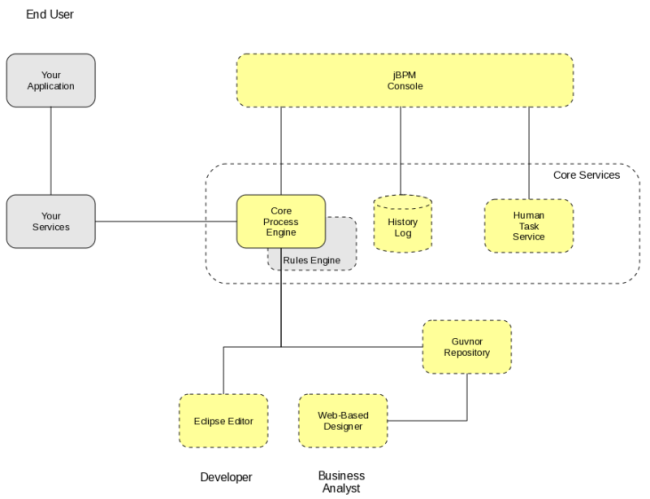
\includegraphics[width=300]{jbpm_overview}
			  \caption[labelInTOC]{Componentes do jBPM}
			  \label{fig:jbpmOverview}
			\end{center}
		\end{figure}
		\FloatBarrier
		
		
	\clearpage	
	\section{Quotero}
	
	Quotero é um sistema de gerenciamento de documentos com código fonte aberto, escrito em Java sob licença GNU GPL
	versão 2. Podemos criar tipos de documentos com campos personalizados ou herdar de outros tipos também, a partir deste
	documentos podemos criar fluxos de trabalho simples, permitindo aplicar um ou mais fluxos de revisões e aprovações para
	os documentos por determinado usuários ou grupos. No andamento do processo um ou mais usuários podem editar o
	documento, preservando sua integridade e reversibilidade com o controle de versões.
	
	O acesso é realizado através de um navegador web em um computador desktop, e também há suporte para acesso com uso de
	um telefone celular. É oferecido um suporte multi idioma para o usuário com traduções em inglês, francês, espanhol e
	polonês.
	
	Através de um plugin, é possível ter integração com Microsoft Office permitindo o usuário criar, abrir e modificar os
	documentos direto do Office, o plugin trata de controlar as versões trabalhadas e trancar o documento enquanto um
	usuário estiver editando para manter sempre a integridade dos documentos.
	
	Todas informações desta seção foram retiradas da referência \cite{QUOTERO}.
	
	

\clearpage
\chapter{Trabalhos relacionados}
		
		\begin{landscape}
			\section{Comparação entre ferramentas}
			%\begin{sidewaystable}[h]
			\begin{table}[h]
			  \centering
			  \tabcolsep=0.11cm
			  \begin{tabular}{|c|c|c|c|c|c|c|c|c|c|}
			    \hline  Nome        	& Linguagem & Licença 		& Indexação de Documentos 	& Controle de versão 	& Workflow 		& ACL 	& LDAP   & OCR				& Escalável  \\
			    \hline  OpenKM      	& Java      & GNU GPL 2		& Sim                		& Sim         			& Sim (jBPM)   	& Sim 	& Sim	 & Sim(Abby OCR)	& Sim		 \\
				\hline  Alfresco     	& Java      & GNU LGPL 2	& Sim                 		& Sim         			& Sim (jBPM)   	& Sim   & Sim	 &					& Sim		 \\
				\hline  Quotero     	& Java      & GNU GPL 2		& Sim                 		& Sim         			& Sim      		& Sim   & Não	 & Não				& Não		 \\
			    \hline  xinco DMS   	& PHP       & 				&                    		&           			&          		&       & 		 &					&			 \\
				\hline  LetoDMS	    	& PHP       & 				& 	                 		&          				&          		&       & 		 &					&			 \\
				\hline  Epiware	    	& 	        & 				& 	                 		&          				&          		&       & 		 &					&			 \\
				\hline  OpenDocMan  	& 	        & 				& 	                 		&          				&          		&       & 		 &					&			 \\
				\hline  Owl 	    	& 	        & 				& 	                 		&          				&          		&       & 		 &					&			 \\
				\hline  Knowledgetree	& 	        & 				& 	                 		&          				&          		&       & 		 &					&			 \\
				\hline  DocMGR			& 	        & 				& 	                 		&          				&          		&       & 		 &					&			 \\
			    \hline  Nuxeo			& 	        & 				& 	                 		&          				&          		&       & 		 &					&			 \\
				\hline  Cuteflow		& 	        & 				& 	                 		&          				&          		&       & 		 &					&			 \\
				\hline
			  \end{tabular}
			  \caption{Tabela Comparativa de Ferramentas DMS}
			\end{table}
			%\end{sidewaystable}
		\end{landscape}


\clearpage
\chapter{Metodologia}



\clearpage
\chapter{Resultados}



\clearpage
\chapter{Conclusão}



\clearpage
%Referências Bibliograficas
\nocite{*}
\bibliographystyle{plain}		
\bibliography{bibliografia}		


\end{document}